\documentclass[dvisvgm,hypertex,aspectratio=169]{beamer}
\usefonttheme{serif}

%\usepackage[draft]{animate}
\usepackage[final]{animate}
\usepackage{ifthen}

\usepackage{khpreamble}


%%%%%%%%%%%%%%%%%%%%%%%%%%%%%%%%%%%%%%%%%%%%%%%%%%%%%%%%%%%%%%%%%%%%%%%%%%%%%%%
% PageDown, PageUp key event handling; navigation symbols
%%%%%%%%%%%%%%%%%%%%%%%%%%%%%%%%%%%%%%%%%%%%%%%%%%%%%%%%%%%%%%%%%%%%%%%%%%%%%%%
\usepackage[totpages]{zref}
\usepackage{atbegshi}
\usepackage{fontawesome}
\setbeamertemplate{navigation symbols}{}
\AtBeginShipout{%
  \AtBeginShipoutAddToBox{%
    \special{dvisvgm:raw
      <defs>
      <script type="text/javascript">
      <![CDATA[
        document.addEventListener('keydown', function(e){
          if(e.key=='PageDown'){
            \ifnum\thepage<\ztotpages
              document.location.replace('\jobname-\the\numexpr\thepage+1\relax.svg');%
            \fi
          }else if(e.key=='PageUp'){
            \ifnum\thepage>1
            %document.location.replace('\jobname-\the\numexpr\thepage-1\relax.svg');%
              document.location.replace('\jobname-\makeatletter\@anim@pad{2}{\thepage-1}\makeatother\relax.svg');%
            \fi%
          }
        });
      ]]>
      </script>
      </defs>
    }%
  }%
  \AtBeginShipoutUpperLeftForeground{%
    \raisebox{-\dimexpr\height+0.5ex\relax}[0pt][0pt]{\makebox[\paperwidth][r]{%
      \normalsize\color{structure!40!}%
      \ifnum\thepage>1%
      \href{\jobname-\the\numexpr\thepage-1\relax.svg}{\faArrowLeft}%
      \else%  
        \textcolor{lightgray}{\faArrowLeft}%  
      \fi\hspace{0.5ex}%
      \ifnum\thepage<\ztotpages%
      \href{\jobname-\the\numexpr\thepage+1\relax.svg}{\faArrowRight}%
      \else%
        \textcolor{lightgray}{\faArrowRight}%  
      \fi%
      \hspace{0.5ex}%
    }}%
  }%  
}%
%%%%%%%%%%%%%%%%%%%%%%%%%%%%%%%%%%%%%%%%%%%%%%%%%%%%%%%%%%%%%%%%%%%%%%%%%%%%%%%

\usepackage{tikz}
\usepackage{pgfplots}
\usepackage{pgfplotstable}
\pgfplotsset{compat=1.16}
\usetikzlibrary{calc}
\usepackage{amsmath}
\DeclareMathOperator{\sign}{sgn}


\author{Kjartan Halvorsen}
\date{2022-05-19}
\title{Mathematical foundations}

% ------------------------------------------------
% Determine which slides to include
\includeonlyframes{%
I0,% Conceptos: ODE, Laplace, transfer fcn
%I1,% Conceptos: ODE, Laplace, transfer fcn
C0,% Control of hummer
L3,% Linealización local ejemplo numerico
CExp,% Exponential function, exercise
LA00,% Laplace
LA1A,% Laplace
LA2A,% Laplace
LA3,% Laplace de derivada
M0,% Modelo de eje flexible.
M1,% FBD, ODE
M2,% Laplace
M3,% Trf fcn
}
% ------------------------------------------------

%%%%%%%%%%%%%%%%%%%%%%%%%%%%%%%%%%%%%%%%%%%%%%%%%%%%%%%%%%%%%%%%%%%%%%%%%%%%%%%
% Define footer
\usepackage{ccicons}

\makeatletter
\setbeamertemplate{footline}
{
  \leavevmode%
  \hbox{%
  %\begin{beamercolorbox}[wd=.333333\paperwidth,ht=2.25ex,dp=1ex,center]{title in head/foot}%
    %\usebeamerfont{title in head/foot}\insertsubsection
  %\end{beamercolorbox}%
  %\begin{beamercolorbox}[wd=.333333\paperwidth,ht=2.25ex,dp=1ex,right]{date in head/foot}%
  %  \usebeamerfont{date in head/foot}\insertshortdate{}\hspace*{2em}
  %  \insertframenumber{} / \inserttotalframenumber\hspace*{2ex} 
  %\end{beamercolorbox}}%
  %\vskip0pt%
  \begin{beamercolorbox}[wd=.92\paperwidth,ht=2.25ex,dp=1ex,right]{author in head/foot}%
    \usebeamerfont{author in head/foot}\insertauthor
  \end{beamercolorbox}%
  \begin{beamercolorbox}[wd=.08\paperwidth,ht=2.25ex,dp=1ex,right]{date in head/foot}%
    \ccbysa
  \end{beamercolorbox}}%
  \vskip0pt%
}
\makeatother
%%%%%%%%%%%%%%%%%%%%%%%%%%%%%%%%%%%%%%%%%%%%%%%%%%%%%%%%%%%%%%%%%%%%%%%%%%%%%%%

\renewcommand*{\laplace}[1]{\ensuremath{\mathcal{L}\big\{ #1 \big\}}}
\renewcommand*{\mexp}[1]{\ensuremath{\mathrm{e}^{#1}}}

\begin{document}

\maketitle


\begin{frame}[label=I0]{Concepts}

  \begin{itemize}
  \item Differential equations
  \item Linearization
  \item The Laplace transform
  \item Transfer functions
  \end{itemize}
  
\end{frame}

%\begin{frame}[label=I1]{Repetición}
%\end{frame}

\begin{frame}[label=C0]{Modeling in the context of automation}
  \footnotesize
  \begin{center}
    \begin{tikzpicture}[scale=0.8, transform shape,
      node distance=2.6cm,
      block/.style={rectangle, draw, minimum height=12mm, minimum width=18mm},
      sumnode/.style={circle, draw, inner sep=1pt},
      ]
      % \useasboundingbox (-1 cm, -1 cm) rectangle (9 cm, 3 cm);
      \pgfmathsetmacro{\xpos}{3}
      \node[anchor=south,] at (\xpos cm, 0) {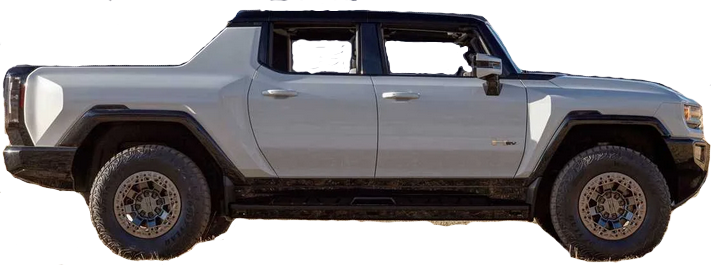
\includegraphics[width=15 mm]{hummer-ev.png}};
      \draw[->, black!90, semithick] (-1, 0.16) -- (9 , 0.16) node[below, pos=1] {};

      \begin{scope}[yshift=-3cm,]
        \node[block] (cc) {Controller};
        \node[sumnode, left of=cc] (sum) {$\Sigma$};
        \node[block, right of=cc, node distance=3cm,] (actuator) {Actuator};
        \node[block, right of=actuator, node distance=3cm,] (plant) {Car};
        \node[block, below of=actuator, node distance=2cm] (sensor) {Sensor};
        \node[coordinate, left of=sum, node distance=2cm] (input) {};
        \node[coordinate, right of=plant, node distance=3cm] (output) {};

        \draw[->] (input) -- node[above, pos=0.2] {$v_{ref}$} (sum);
        \draw[->] (sum) -- node[above, ] {$e$} (cc);
        \draw[->] (cc)  -- (actuator);
        \draw[->] (actuator) -- node[above, ] {$T_m$} (plant);
        \draw[->] (plant)  -- node[coordinate] (meas) {} node[above, pos=0.9] {$v$} (output);
        \draw[->] (meas) |- node[above, ] {} (sensor);
        \draw[->] (sensor) -| node[left, pos=0.95 ] {$-$} (sum);
      \end{scope}
      
    \end{tikzpicture}
  \end{center}
\end{frame}

\note{%
  1) El tema de la materia es la busceda de modelos matematicos para sistemas dinamicas. De modelos que son  adecuados para el desarrollo de sistemas de control o automatización. Ser adecuado significa que el modelo describe las caracteristicas dinamicas más prominentes del sistema.
  2) El ejemplo que vimos el lunes era de un modelo del comportamiento de un coche, en el contexto de un controlador de velocidad. Un cruise control.
  3) En el sistema la señal de salida interesante del coche es su velocidad, que se mide con on sensor y se utiliza en el controlador, comparando con una velocidad desada. El controlador determine un señal adecuada en cada momento a mandar al motor/actuador. El motor (incluyendo la cadena de transmission) cuasa una fuerza F_m en el coche.
  4) Para poder utilizar métodos podorosos para diseñar un controlador y para analizar el sistema en lazo cerrado, buscamos un modelo dinamico LINEAL del coche.
  5) Modelos dinamicos lineales son ellos QUE SE PUEDEN EXPRESAR COMO UNA FUNCIÓN DE TRANSFERENCIA en el dominio de laplace.
}


\begin{frame}[label=I1]{Point-mass model}

  Newton's second law: ``The rate of change of the momentum is equal to the sum of forces''
  \[ \frac{d}{dt} (mv) = \sum_i F_i\]
  \begin{columns}
    \begin{column}{0.7\linewidth}
  \begin{center}
    \footnotesize
    \begin{tikzpicture}[scale=0.6, transform shape]
      \node[anchor=south,] at (1, 0) (hummer) {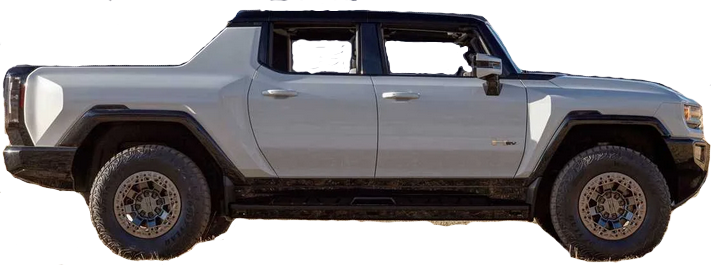
\includegraphics[width=15 mm]{hummer-ev.png}};
      \node[coordinate] (com) at ($ (hummer.center) + (0.15, 0) $) {};
      \node[coordinate] (wheels) at ($ (hummer.south) + (0, 0.16) $) {};
      
      \draw[->, black!90, semithick] (-1, 0.16) -- (9 , 0.16) node[below, pos=1] {$X$};
      \draw[->, black!90, ] (-1, 0.16) -- (-1 , 3) node[left, pos=1] {$Y$};
      
      \draw[thick, green!70!black, ->] (com) -- ++(0, -2cm) node[right] {$F_g = mg$};
      \draw[thick, orange!80!black, ->] (wheels) -- ++(0, 2cm) node[right] {$F_{n}$};
      \draw[thick, red!80!black, ->] (wheels) -- ++(2cm, 0) node[below] {$F_m$};
      \draw[thick, blue!80!black, <-] (hummer.east) -- ++(2cm, 0) node[above] {$F_d$};

    \end{tikzpicture}
  \end{center}

  \[ m\dot{v} = F_m - \sign(v)(r + kv^2)\]
\end{column}
\begin{column}{0.3\linewidth}
  \pause

  \[\sign(v) = \begin{cases} 1, & v > 0\\ 0, & v=0\\-1, & v<0 \end{cases}\]
\end{column}
\end{columns}
\end{frame}

\note{%
  - Viendo el coche como un masa puntual, u aplicando la segunda ley de Newton llegamos a ese ecuación diferencial.
  - La masa por la acceleracion es igual a la suma de las fuerzas. Las fuerzas son la fuerza del motor y el arrastre.
  - El arrastre consiste en dos partes. 1) La resistencia a la rodadura, que es constante. Y 2) la resistencia al aire que crece con la velocidad cuadrada. El arrastre trabaja en contra del movimiento del coche, y claramente cambia signo cuando la velocidad cambia signo. Por eso está la función de signo. 
  - Este es la función de signo. Se necesita para que el arrastre 
}
\begin{frame}[label=L2A]{Linearization}
  \footnotesize
  \begin{columns}
    \begin{column}{0.6\columnwidth}
      \begin{description}
        \item[Define an operating point \(v_0\)  and a deviation variable \(y\)]
          \[ v(t) = v_0 + y(t) \quad \Leftrightarrow \quad y(t) = v(t) - v_0\]
          \pause
        \item[Aproximate the function using its Taylor series]
          \begin{align*}
        F_d=f(v) &= \sign(v)(r + kv^2) = \begin{cases} r + kv^2, & v\ge 0\\-r-kv^2, & v<0 \end{cases}\\
             &\approx f(v_0) + \frac{df}{dv}\big|_{v_0}\underbrace{(v - v_0)}_y\\
        \frac{df}{dv} &= \begin{cases} 2kv, & v>0\\-2kv, & v<0\\\text{undefined}, & v=0 \end{cases}
      \end{align*}
          \pause
      \item[Substitute the approximation in the differential equation]
      \begin{align*}
        m\frac{d}{dt} v &= m\frac{d}{dt} (v_0 + y) = m\frac{d}{dt} y = F_m - F_d\\
        &\approx F_m - f(v_0) - \frac{df}{dv}\Big|_{v=v_0} y
        = -2kv_0y + \overbrace{\big(F_m - f(v_0)\big)}^u.
      \end{align*}
    \end{description}
  \end{column}

    \begin{column}{0.4\columnwidth}
    \begin{center}
    \begin{animateinline}[controls, palindrome]{2}
      \multiframe{3}{n=2+0.44}{
        \begin{tikzpicture}[scale=0.8]
        \pgfmathsetmacro{\vnull}{\n}
        \pgfmathsetmacro{\Fnull}{sign(\vnull)*(0.4+\vnull*\vnull)}
          \begin{axis}[
            axis lines = middle,
            ytick={\Fnull},
            yticklabels={$f(v_0)$},
            xtick={\vnull},
            xticklabels={$v_0$},
            xlabel={$v$},
            ylabel={$F_d$},
            clip=false,
            xmin=-6,
            xmax=6,
            ymin=-20,
            ymax=20,
            ]
           
            \addplot [blue!80, domain=-4:4, samples=400, thick] { sign(x)*(1 + x*x)};
            %\addplot [orange!80, domain=-1.5:1.5, samples=4, variable=\t] ({t}, {t});
            \addplot [orange!80, domain=-1.5:1.5, samples=4, variable=\t, thick] ({t+\vnull}, {sign(\vnull)*(1 + pow(\vnull, 2)) + (2*abs(\vnull))*t} );
          \end{axis}
        \end{tikzpicture}
      }
    \end{animateinline}
  \end{center}
\begin{description}
          \pause
  \item[Linearized differential equation]
    \[m\dot{y} = -2kv_0y + u\]
  \end{description}
\end{column} 
\end{columns}
\end{frame}

\note{%
  - El arrastre es una función nonlineal de la velocidad v.
  - Estamos buscando una función lineal aproximada de esta función.
  - Cada función suave (analitica) se puede approximar arbitrariamente bien alrededor de un punto con una serie de potencias convergentes. Es decir que tiene un serie de Taylor convergente. Usamos solamente la parte lineal de la serie de Taylor.
  - 1) Eligimos el punto de operación. Es decir una velocdad tipica, por ejemplo 80 km/h. El modelo va a ser preciso cerca de 80, pero no a 40 o 120 km/h
  - 2) Definimos una variable de desviación.
  - 3) El valor de la función se aproxima como su valor en el punto de operación más la inclinación del tangente por el valor de la variable de desviación.
  - 4) La inclinación del tangente es la derivada de la función en ese punto (el punto de desviación)
  - 5) Substituir la aproximación lineal en la ED original. 
  - 6) 
}


\begin{frame}[label=CExp]{The complex exponential function \(f(t) = r\mathrm{e}^{\lambda t}, \quad \lambda\in\mathbb{C} \)}
  \footnotesize
  
  \[ t \in \mathbb{R_+}, \qquad \lambda = a + i\omega \in \mathbb{C}, \qquad r \in \mathbb{R}  \]
  \[ f: \mathbb{R_+} \mapsto \mathbb{C}, \qquad f(t) = r\mathrm{e}^{\lambda t} = r\mathrm{e}^{at}\mathrm{e}^{i\omega t} = r\mathrm{e}^{at}\big(\cos(\omega t) + i\sin(\omega t)\big), \qquad 0 < t < \infty \]

  \pause

  Match the value of the parameter $\lambda$ with the correct time-function (showing the real-part of the function). Let $r=1$.

  \begin{center}
    \begin{tabular}{cccc}
      \textcolor{blue!80!black}{A} & \textcolor{blue!80!black}{B} & \textcolor{blue!80!black}{C} & \textcolor{blue!80!black}{D}\\ 
      \(\quad\lambda = 2i\quad\) &       \(\quad\lambda = 1-2i\quad\) &       \(\quad \lambda = -1+2i \quad \) &    \(\quad \lambda = -1\quad \)
    \end{tabular}
  \end{center}

  \begin{center}
    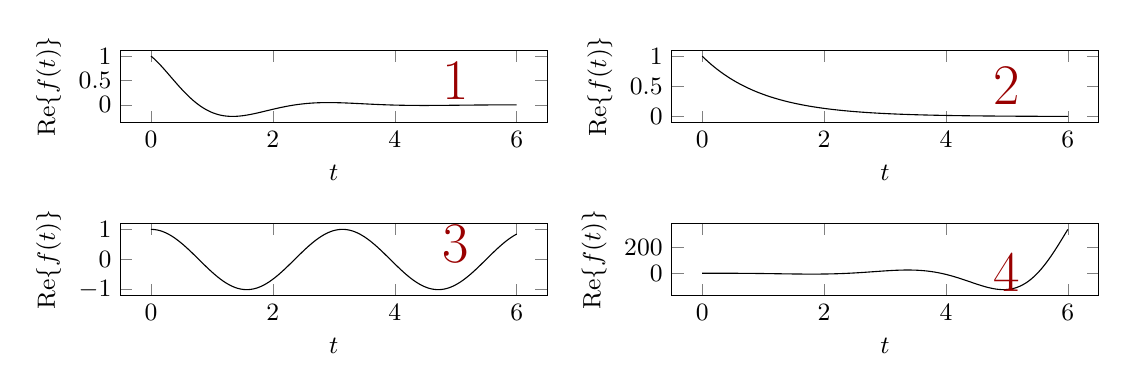
\begin{tikzpicture}
      \small
      % Order 3421

      \def\aone{0}
      \def\atwo{1}
      \def\athree{-1}
      \def\afour{-1}

      \def\wone{2}
      \def\wtwo{-2}
      \def\wthree{2}
      \def\wfour{0}
      
      \begin{axis}[
        width=7cm,
        height=2.5cm,
        xlabel={$t$},
        ylabel={$\mathrm{Re}\{f(t)\}$},
        xmin=-0.5,
        xmax=6.5,
        %ytick = {0},
        %xtick = {0},
        %xticklabels = {$t_1$},
        ]
        \addplot+[black, no marks, domain=0:6, samples=400,variable=k] {
          exp(\athree * k)*cos((180/3.1416) * \wthree * k))};
        \node[black!40!red] at (axis cs: 5, 0.5) {\huge 1};
      \end{axis}

      \begin{axis}[
        xshift=7cm,
        width=7cm,
        height=2.5cm,
        xlabel={$t$},
        ylabel={$\mathrm{Re}\{f(t)\}$},
        xmin=-0.5,
        xmax=6.5,
        %ytick = {0},
        %xtick = {0},
        %xticklabels = {$t_1$},
        ]
        \addplot+[black, no marks, domain=0:6, samples=400,variable=k] {
          exp(\afour * k)*cos((180/3.1416) * \wfour * k))};
        \node[black!40!red] at (axis cs: 5, 0.5) {\huge 2};
      \end{axis}

      \begin{axis}[
        xshift=0cm,
        yshift=-2.2cm,
        width=7cm,
        height=2.5cm,
        xlabel={$t$},
        ylabel={$\mathrm{Re}\{f(t)\}$},
        xmin=-0.5,
        xmax=6.5,
        ]
        \addplot+[black, no marks, domain=0:6, samples=400,variable=k] {
          exp(\aone * k)*cos((180/3.1416) * \wone * k))};
        \node[black!40!red] at (axis cs: 5, 0.5) {\huge 3};
      \end{axis}

      \begin{axis}[
        xshift=7cm,
        yshift=-2.2cm,
        width=7cm,
        height=2.5cm,
        xlabel={$t$},
        ylabel={$\mathrm{Re}\{f(t)\}$},
        xmin=-0.5,
        xmax=6.5,
        ]
        \addplot+[black, no marks, domain=0:6, samples=400,variable=k] {
          exp(\atwo * k)*cos((180/3.1416) * \wtwo * k))};
        \node[black!40!red] at (axis cs: 5, 0.5) {\huge 4};
      \end{axis}


    \end{tikzpicture}

  \end{center}

\end{frame}

  \begin{frame}[label=LA00]{The Laplace transform}

    \[ F(s) = \laplace{f(t)} = \int_0^\infty f(t)\mexp{-st}dt\]
    \pause
    \[ f(t) = \laplaceinv{F(s)} = \frac{1}{2\pi i} \lim_{T\to\infty} \int_{\gamma-Ti}^{\gamma + Ti} e^{st}F(s) ds \]
    \pause
    
    \begin{center}
      \begin{tikzpicture}[scale=0.8]
        \draw[thick, ->] (-7, 0) -- node[very near end, below] {$t$} (-1, 0);
        \draw[] (-6, 0) -- (-6, -0.1) node[below] {0};
        \begin{scope}[xshift=-6 cm,]
          \draw[blue!80, domain=-1:4, samples=220] plot (\x, {(\x>0)*2*exp(-2*\x)});
        \end{scope}
        \draw[thick, ->] (1, 0) -- node[very near end, below] {Re} (7, 0);
        \draw[thick, ->] (4,-3) -- node[very near end, left] {Im} (4, 3);
        \node at (5, 3) {$s$-plane};
        \node[orange!80] at (2, 0) {\huge $\times$}; 

        \draw[->] (-0.5, 1) arc [start angle=150, end angle=30, radius=0.5 cm] node[pos=0.5, above] {$\mathcal{L}$};
        \draw[->] (0.5, -1) arc [start angle=-30, end angle=-150, radius=0.5 cm] node[pos=0.5, below] {$\mathcal{L}^{-1}$};
      \end{tikzpicture}
    \end{center}

  \end{frame}

  \begin{frame}[label=LA1A]{The Laplace transform}

    \[F(s) = \laplace{f(t)} = \int_0^\infty f(t)\mexp{-st}dt\]
    \[\laplace{\mexp{pt}} = \int_0^\infty \mexp{pt}\mexp{-st}dt = \int_0^\infty \mexp{-(s-p)t}dt = \frac{1}{s-p}, \quad \mathrm{Re}\{s\} > \mathrm{Re}\{p\} \]

\begin{center}
      \begin{animateinline}[controls,]{2}
        \multiframe{7}{n=1+1}{
          \begin{tikzpicture}[scale=0.7,]
            \pgfmathsetmacro{\aa}{-2.5 + 0.5*\n}
          \begin{axis}[%
            width=6.5cm,
            height=3.5cm,
            axis lines = middle,
            ytick=\empty,
            xtick=\empty,
            xlabel={$t$},
            ylabel={$f$},
            xmin=-0.5,
            xmax=6,
            %ymax=1.4,
            ]
            \addplot [blue!80, domain=-1:6, samples=300, thick] { (x>=0)*exp(\aa*x) };
          \end{axis}

             \begin{scope}[xshift=9cm, yshift=1cm]
            \node {\includegraphics[width=5cm]{laplace-real-\n.png}};
            %  \node {\aa};
            \end{scope}
          \end{tikzpicture}
        }
      \end{animateinline}
    \end{center}
  \end{frame}
  
  \begin{frame}[label=LA2A]{The Laplace transform}

    \[F(s) = \laplace{f(t)} = \int_0^\infty f(t)\mexp{-st}dt\]
    \[\laplace{\sin(\omega_1 t)} = \int_0^\infty \frac{1}{2i} \big( \mexp{i\omega_1t} + \mexp{-i\omega_1 t}\big)\mexp{-st}dt = \frac{\omega}{(s-i\omega_1)(s+i\omega_1)}, \quad \mathrm{Re}\{s\}>0 \]

\begin{center}
      \begin{animateinline}[controls,]{2}
        \multiframe{5}{n=2+1}{
          \begin{tikzpicture}[scale=0.7,]
            \pgfmathsetmacro{\ww}{0.5 + 0.5*(\n-2)}
          \begin{axis}[%
            width=6.5cm,
            height=3.5cm,
            axis lines = middle,
            ytick=\empty,
            xtick=\empty,
            xlabel={$t$},
            ylabel={$f$},
            xmin=-0.5,
            xmax=6,
            %ymax=1.4,
            ]
            \addplot [blue!80, domain=-1:6, samples=300, thick] { (x>=0)*sin(100*\ww*x) };
          \end{axis}

             \begin{scope}[xshift=9cm, yshift=1cm]
            \node {\includegraphics[width=5cm]{laplace-imag-\n.png}};
            %  \node {\aa};
            \end{scope}
          \end{tikzpicture}
        }
      \end{animateinline}
    \end{center}
  \end{frame}

    \begin{frame}[label=LA3]{The Laplace transform of a derivative}
      \small
      \[F(s) = \laplace{f(t)} = \int_0^\infty f(t)\mexp{-st}dt\]

  %   {\scriptsize
  %   Using integration by parts
  %   \[ \frac{d}{dt}(uv) = (\frac{d}{dt} u) v + u (\frac{d}{dt}) v \]
  %   \[ \int (\frac{d}{dt} u) v dt  = \int \frac{d}{dt}(uv) dt - \int u (\frac{d}{dt} v ) dt \]
  % }

  % \begin{align*}
  %     \laplace{\frac{d}{dt}f(t))} &= \int_0^\infty (\frac{d}{dt}f(t))\mexp{-st}dt\\
  %     \end{align*}
  % \begin{align*}
  %     \laplace{\frac{d}{dt}f(t))} &= \left[f(t)\mexp{-st}\right]_0^\infty - \int_0^\infty f(t)(-s\mexp{-st})dt\\
  %                                 &= sF(s) - f(0).
  %   \end{align*}

  \begin{align*}
      \laplace{\frac{d}{dt}f(t))} &=  sF(s) - f(0).
  \end{align*}

    \end{frame}

    \begin{frame}[label=L3]{Linearized model of the Hummer EV}

    \footnotesize

    Parameters: $m$=5000kg, $C_d$=0.6, $A$=\unit{4}{\meter\squared}, $C_{rr}$=0.01

  \begin{columns}
    \begin{column}{0.6\linewidth}

      \begin{align*}
        F_d(v) &= r + kv^2 = C_{rr}mg + \frac{1}{2}\rho_a C_d A v^2\\
               &= 0.01\cdot 5000\cdot9.8 + \frac{1}{2}1.2\cdot 0.6\cdot 4 v^2 = 490 + 1.44v^2.
      \end{align*}
      
      \begin{description}
        \pause
      \item[Operating point and deviation variables]
        $v_0 = \unit{22}{\meter\per\second}$, $v(t)=v_0 + y(t)$, $F_m(t) = F_{m_0} + u(t) = F_d(v_0) + u$ 
        \pause
      \item[Linearized ODE]
    \[m\dot{y} = -2kv_0y + u,\]
    \[ \dot{y} + \frac{2\cdot 1.44\cdot 22}{5000} y = \frac{1}{5000} u, \]
    \[ \dot{y} + 0.013 y = 0.0002u, \]
    \[ 78.9\dot{y} + y = 0.016u. \]
        \pause
  \end{description}
\end{column}
\begin{column}{0.4\linewidth}
  \begin{description}
  \item[The Laplace transform]
    \[ (78.9s + 1) Y(s) = 0.016 U(s) \]
        \pause
  \item[Transfer function]
    \[  Y(s) = \underbrace{\frac{\overbrace{0.016}^K}{ \underbrace{78.9}_\tau s + 1}}_{G(s)} U(s) \]

        \pause
  \item[Block diagram]
  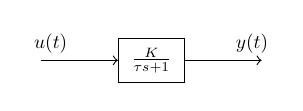
\begin{tikzpicture}[scale=0.7, transform shape, block/.style={draw, minimum width=12mm, minimum height=8mm},]
    \node[block] (plant) {$\frac{K}{\tau s + 1}$};
    \draw[->] (plant) ++ (-2cm, 0) -- node[very near start, above] {$u(t)$} (plant);
    \draw[->] (plant) -- node[very near end, above] {$y(t)$} ++(2cm, 0);
  \end{tikzpicture}
\end{description}
\end{column}
\end{columns}
\end{frame}

  \begin{frame}[label=M0]{Modeling a mechanical system}
    \small

    \begin{center}
      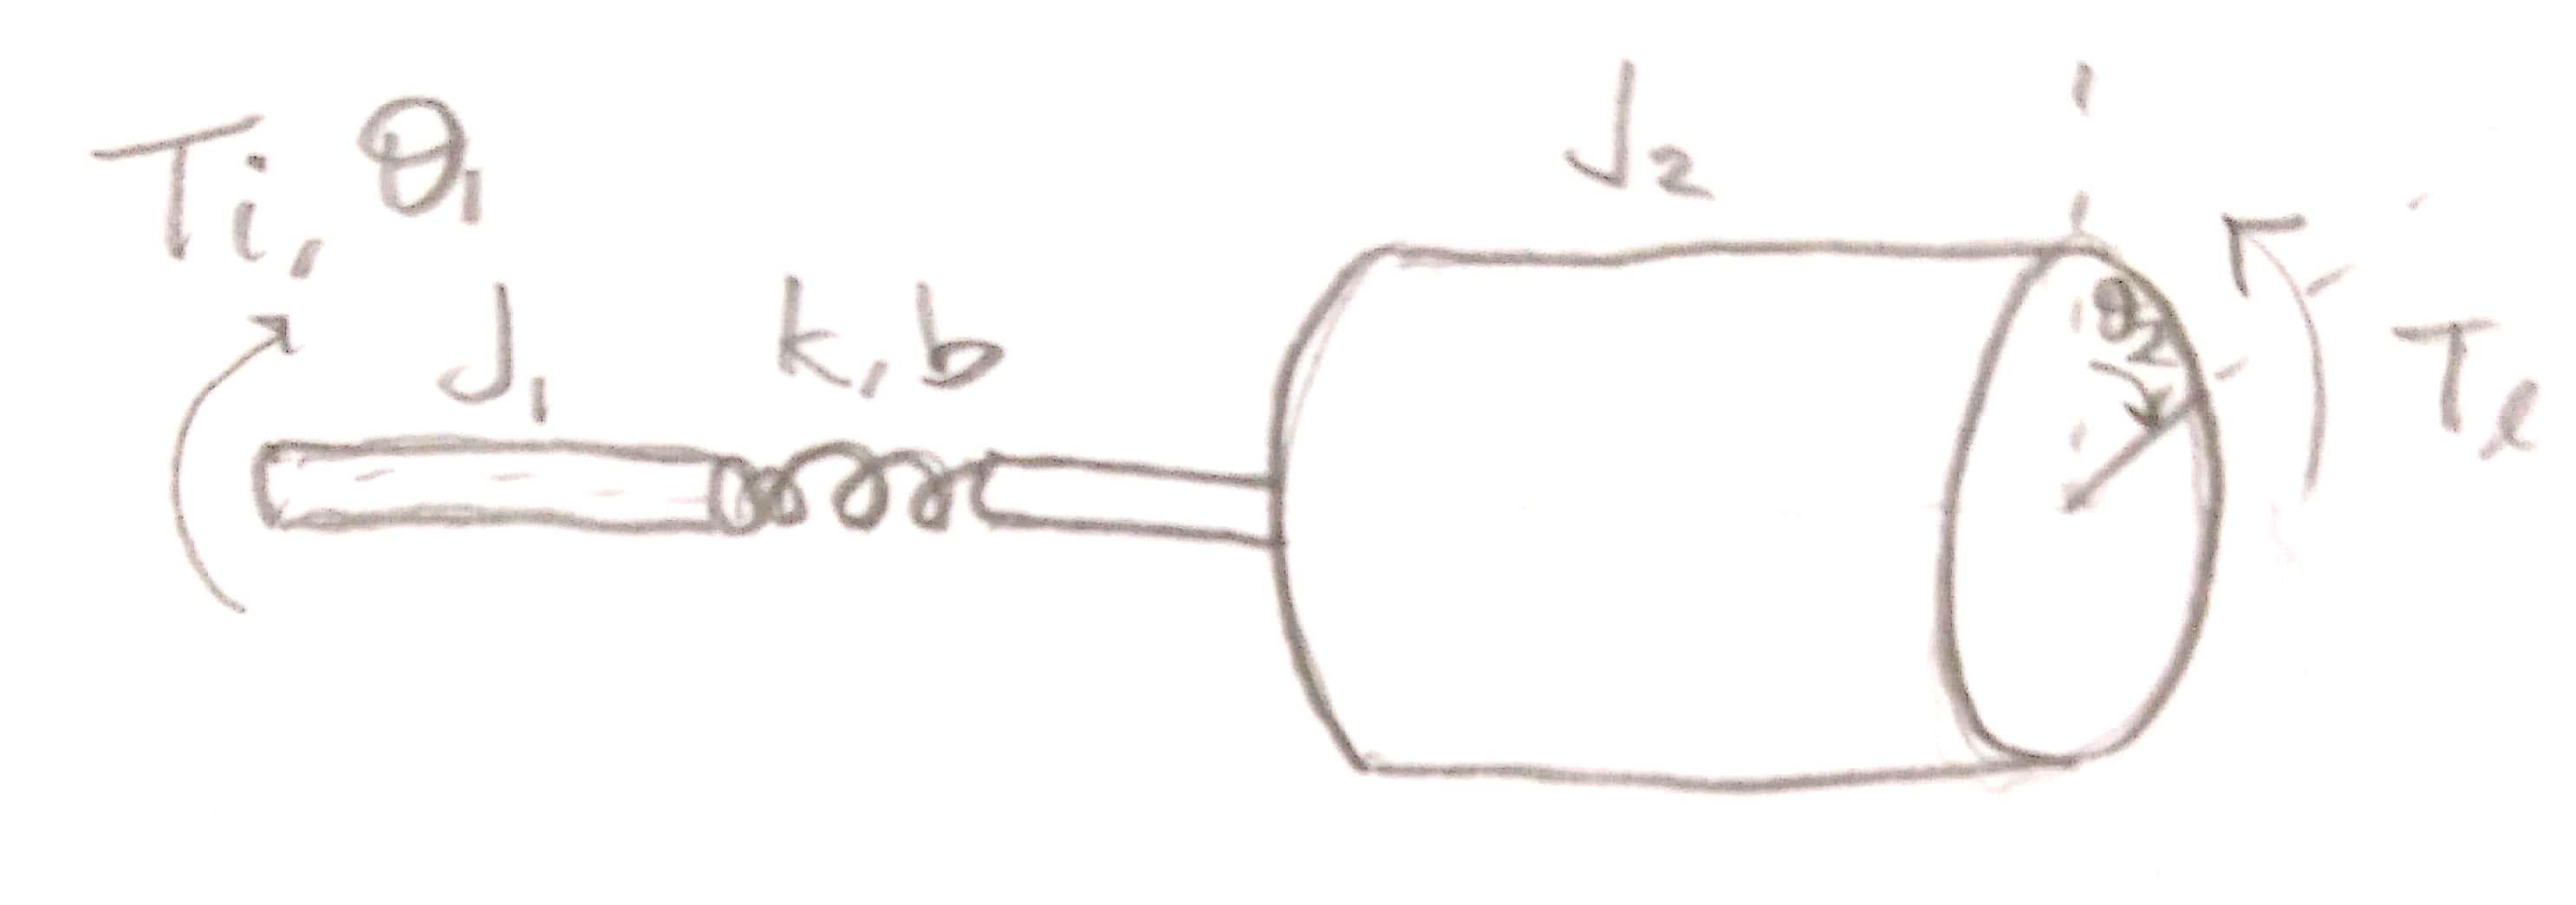
\includegraphics[width=0.4\linewidth]{elastic-shaft.jpg}
      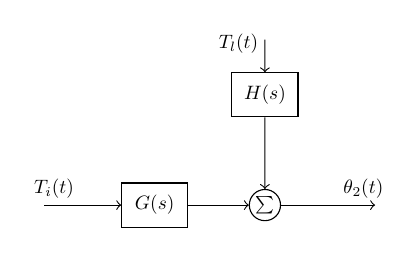
\begin{tikzpicture}[scale=0.7, transform shape, block/.style={draw, minimum width=12mm, minimum height=8mm},]
        \node[block] (plant) {$G(s)$};
        \node[circle, draw, inner sep=1pt, right of=plant, node distance=2cm] (sum) {\small $\sum$};
        \node[block, above of=sum, node distance=2cm] (load) {$H(s)$};
        \draw[->] (plant) ++ (-2cm, 0) -- node[very near start, above] {$T_i(t)$} (plant);
        \draw[->] (load) ++ (0,1cm) -- node[very near start, left] {$T_l(t)$} (load);
        \draw[->] (plant) -- (sum);
        \draw[->] (load) -- (sum);
        \draw[->] (sum) -- node[very near end, above] {$\theta_2(t)$} ++(2cm, 0);
      \end{tikzpicture}\\
      A motor drives a load via an elastic shaft. Determine the transfer functions $G(s)$ and $H(s)$.
    \end{center}

\end{frame}


  \begin{frame}[label=M1]{Modeling a mechanical system}
    \small

    \begin{center}
      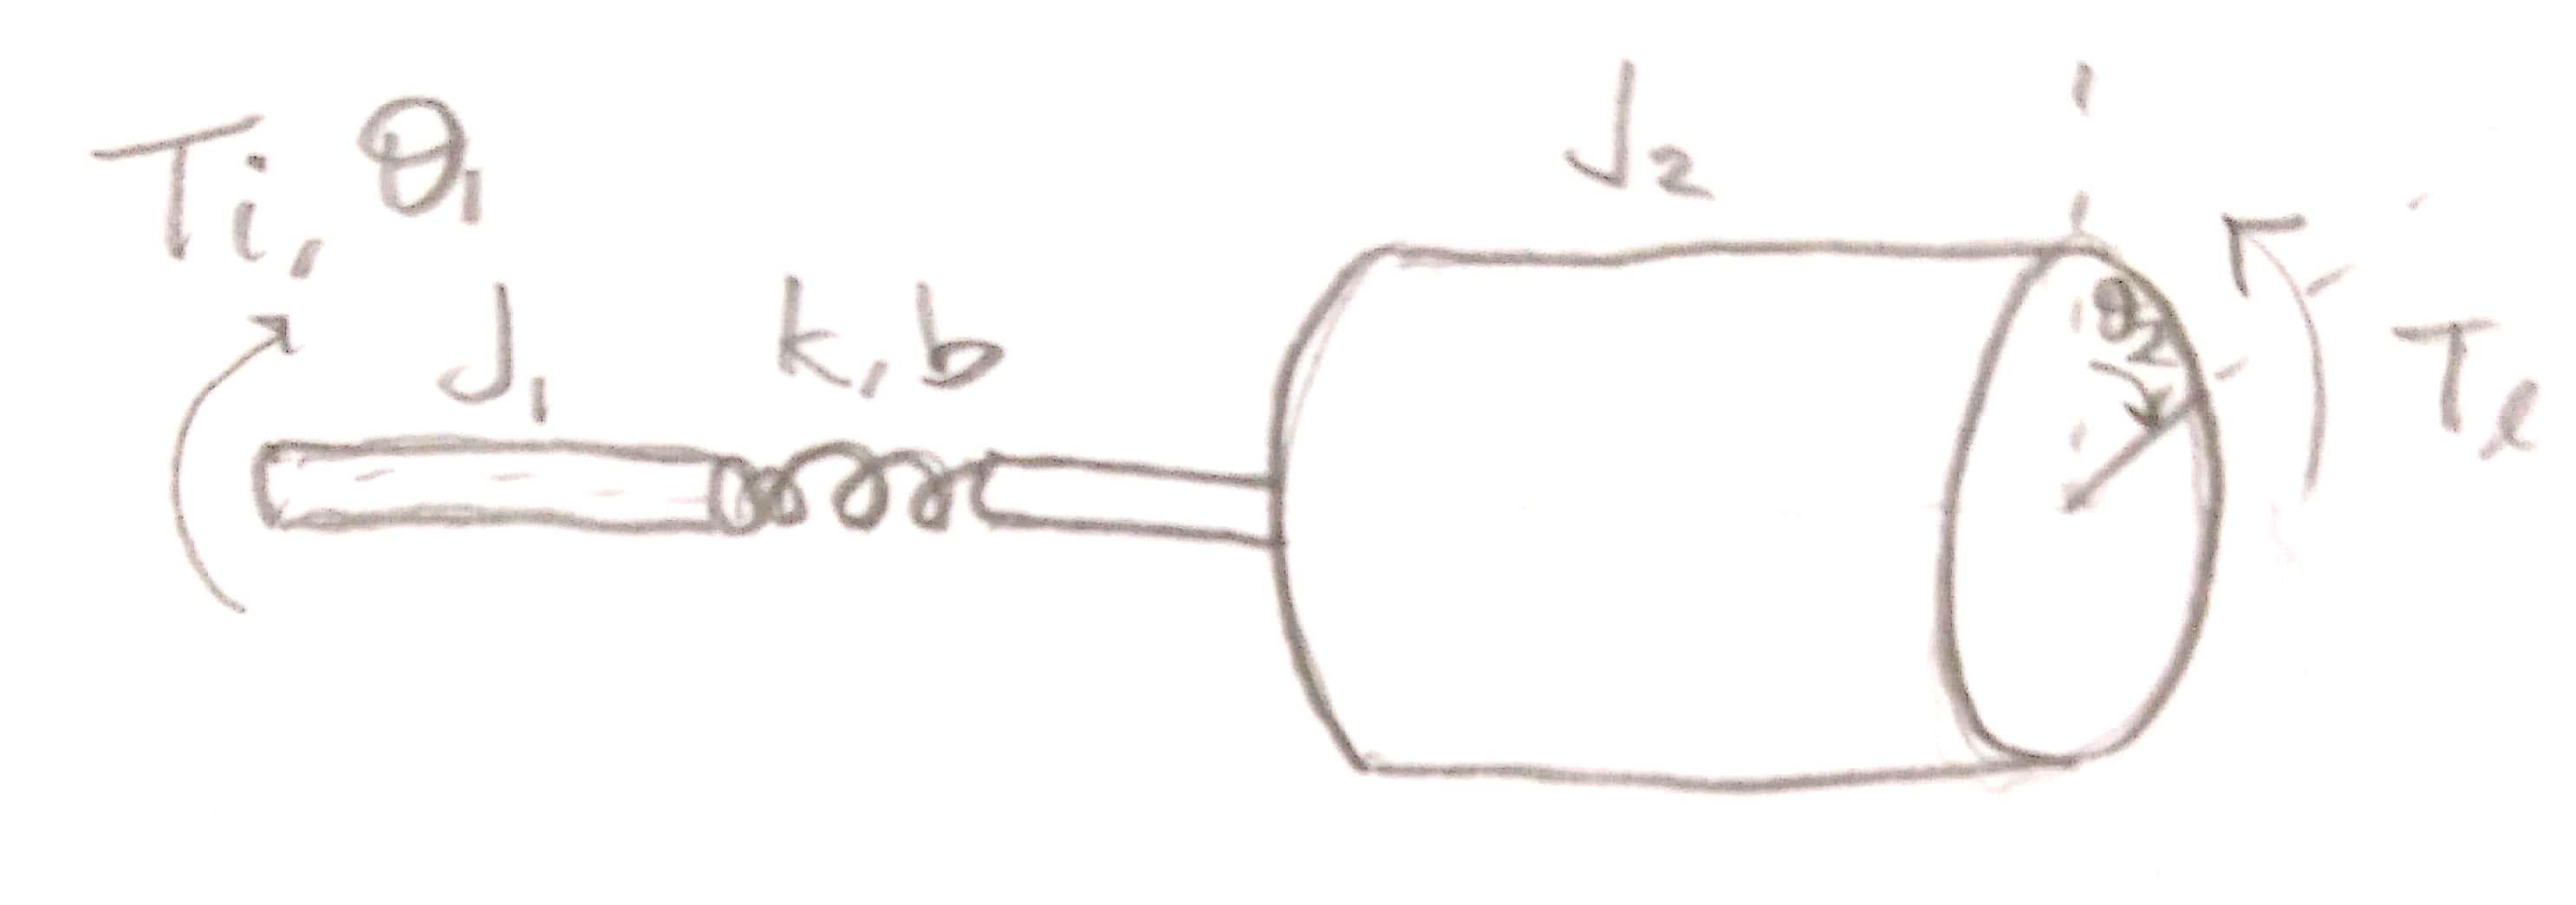
\includegraphics[width=0.3\linewidth]{elastic-shaft.jpg}
      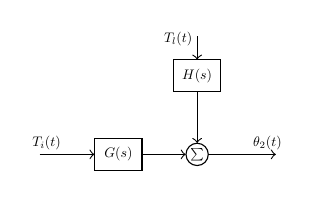
\begin{tikzpicture}[scale=0.5, transform shape, block/.style={draw, minimum width=12mm, minimum height=8mm},]
        \node[block] (plant) {$G(s)$};
        \node[circle, draw, inner sep=1pt, right of=plant, node distance=2cm] (sum) {\small $\sum$};
        \node[block, above of=sum, node distance=2cm] (load) {$H(s)$};
        \draw[->] (plant) ++ (-2cm, 0) -- node[very near start, above] {$T_i(t)$} (plant);
        \draw[->] (load) ++ (0,1cm) -- node[very near start, left] {$T_l(t)$} (load);
        \draw[->] (plant) -- (sum);
        \draw[->] (load) -- (sum);
        \draw[->] (sum) -- node[very near end, above] {$\theta_2(t)$} ++(2cm, 0);
      \end{tikzpicture}\\

    \end{center}

    Newton's second law for rotational systems
      \[ J\ddot{\theta} = \sum_j T_j \]

      \begin{description}
        \pause
      \item[Free-body diagram]
          \begin{align*}
            \text{Body 1:}\qquad & J_1 \ddot{\theta}_1 = T_i - k (\theta_1 - \theta_2) - b(\dot{\theta}_1 - \dot{\theta}_2)\\
            \text{Body 2}: \qquad & J_2 \ddot{\theta}_2 = k (\theta_1 - \theta_2) - b(\dot{\theta}_1 - \dot{\theta}_2) - T_l
          \end{align*}
        \pause
       \item[Apply Laplace]
      \begin{align*}
        J_1s^2\Theta_1 + bs\Theta_1 + k\Theta_1 = k\Theta_2 + bs\Theta_2 + T_i \quad &\Leftrightarrow\quad (J_1s^2 + bs + k)\Theta_1 = (k + bs) \Theta_2 + T_i\\ 
        J_2s^2\Theta_2 + bs\Theta_2 + k\Theta_2 = k\Theta_1 + bs\Theta_1 - T_l  \quad &\Leftrightarrow\quad  (J_2s^2 + bs + k)\Theta_2 = (k + bs) \Theta_1 - T_l
      \end{align*}
    \end{description}
\end{frame}

  \begin{frame}[label=M2]{Modeling a mechanical system}

    \begin{center}
      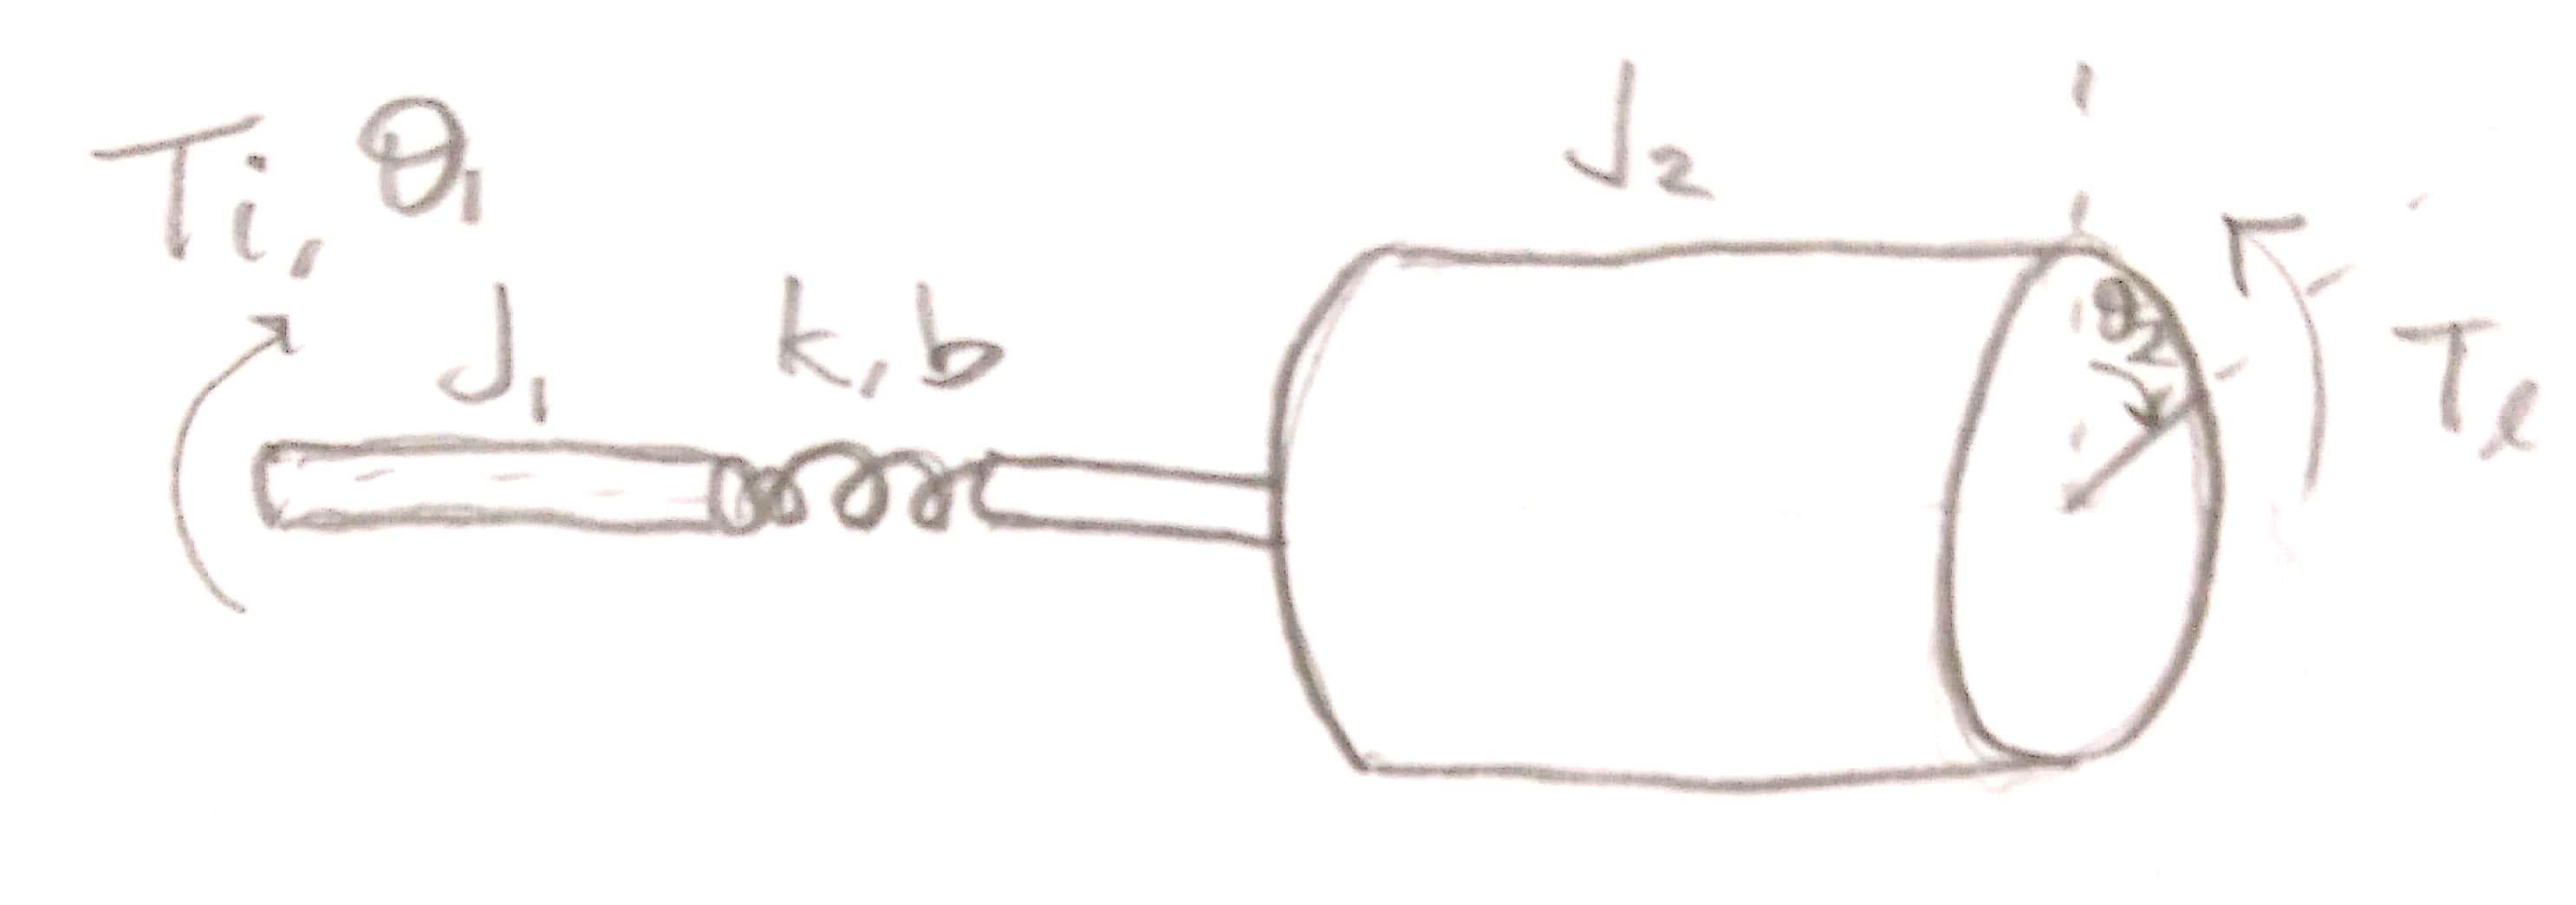
\includegraphics[width=0.3\linewidth]{elastic-shaft.jpg}
      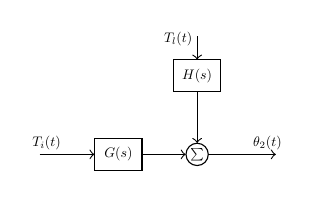
\begin{tikzpicture}[scale=0.5, transform shape, block/.style={draw, minimum width=12mm, minimum height=8mm},]
        \node[block] (plant) {$G(s)$};
        \node[circle, draw, inner sep=1pt, right of=plant, node distance=2cm] (sum) {\small $\sum$};
        \node[block, above of=sum, node distance=2cm] (load) {$H(s)$};
        \draw[->] (plant) ++ (-2cm, 0) -- node[very near start, above] {$T_i(t)$} (plant);
        \draw[->] (load) ++ (0,1cm) -- node[very near start, left] {$T_l(t)$} (load);
        \draw[->] (plant) -- (sum);
        \draw[->] (load) -- (sum);
        \draw[->] (sum) -- node[very near end, above] {$\theta_2(t)$} ++(2cm, 0);
      \end{tikzpicture}\\
    \end{center}
    \scriptsize
    \begin{description}
    \item[Eliminate the variable \(\Theta_1\)]
      Substitute \(\Theta_1 = \frac{k+bs}{J_1s^2 + bs + k}\Theta_2 + \frac{1}{J_1s^2 + bs + k}T_i\) 
      in the equation \[(J_2s^2 + bs + k)\Theta_2 = (k + bs) \Theta_1 - T_l\]
      {\tiny
      \begin{align*}
        (J_2s^2 + bs + k)\Theta_2 &= (k+bs) \left(\frac{k + bs}{J_1s^2 + bs + k} \Theta_2 + \frac{1}{J_1s^2 + bs + k}T_i\right) - T_l\\
        (J_2s^2 + bs + k)\Theta_2  &- \frac{(k+bs)^2}{J_1s^2 + bs + k}\Theta_2 = \frac{k+bs}{J_1s^2 + bs + k} T_i - T_l\\
        \frac{(J_2s^2 + bs +k)(J_1s^2 + bs + k) - (k+bs)^2}{J_1s^2 + bs + k} \Theta_2 &= \frac{k+bs}{J_1s^2 + bs + k} T_i - T_l\\
        \frac{J_2J_1s^4 + (J_1+J_2)s^2(bs +k)}{J_1s^2 + bs + k} \Theta_2 &= \frac{k+bs}{J_1s^2 + bs + k} T_i - T_l\\
        \Theta_2(s) &= \underbrace{\frac{k + bs}{s^2(J_1J_2s^2 + bs + k)}}_{G(s)}T_i(s) \underbrace{- \frac{J_1s^2 + bs + k}{s^2(J_1J_2s^2 + bs + k)}}_{H(s)}T_l(s)
      \end{align*}}
    \end{description}      
  \end{frame}
\end{document}


